\section{Theoretical Analysis}
\label{sec:analysis}



\subsection{Node Analysis ($t<0$)}

In this particular section, the circuit is analysed in $t<0$, therefore, we can apply the usual node analysis, with no sinusoidal tensions in the voltage source Vs: for $t<0$ $v_s = Vs$.

Labels were assigned to identify nodes from zero to eight (no node four given in instructions), and directions to currents as seen in figure (\ref{FIGURA}), to then proceed with the node analysis.  We can, therefore, derive direct equations in terms of the voltage at these nodes.

For this procedure, one applies KCL (Kirchoff's Current Law), which states that the sum of currents leaving a node must be the same as the sum of currents entering a node. Because this kind of approach is only possible for the nodes which aren't directly connected to a terminal of a voltage source, it's crucial to find other equations to cover all the unknown variables of the system. In this case, it's important to consider factor like the voltage gain between two nodes separated by a voltage source: for example, from nodes 0 and 1, the terminals of $v_s$, we can take the equation: $V_1 = V_0 + V_s$. As $V_0$ is identified as the ground ($V_0 = 0V$) we're left with: $V_1 = V_s$.

Moreover, we can relate the currents associated with the current or voltage controlled sources with the nodes voltages, giving us two more equations, the nineth and thenth.

The equations are as follows:

\begin{equation} 
\begin{cases}

    Node\, 0: V_0 = 0 \\
    Node\, 1: V_1 = V_s \\
    Node\, 2: \frac{V_1 - V_2}{R_1} + \frac{V_3 - V_2}{R_2} - \frac{V_2 - V_5}{R_3} = 0 \\
    Node\, 3: -\frac{V_3 - V_2}{R_2} + I_b = 0 \\
    Node\, 5: V_5 - V_8 = V_d \\
    Node\, 6: \frac{V_5 - V_6}{R_5} - I_b = 0 \\
    Node\, 7: \frac{V_0 - V_7}{R_6} - \frac{V_7 - V_8}{R_7} = 0 \\
    Supernode\, 5-8: \frac{V_2 - V_5}{R_3} - \frac{V_5 - V_6}{R_5} + \frac{V_7 - V_8}{R_7} - \frac{V_5 - V_0}{R_4} = 0 \\
    I_d = \frac{V_0 - V_7}{R_6} \\
    I_b = K_b\,(V_2 - V_5) \\
    
\end{cases}
\label{eq:1}
\end{equation}


Note that as there's no sinusoidal excitation ($v_s = constant$), the capacitor behaves like an open circuit and so the current $I_c$ is null and not included in the equations, because:

\begin{center}
  \begin{equation}
    I_c = C\frac{dv}{dt}
  \end{equation}
\end{center}


Using \textit{GNUOctave}, we computed the values of the node voltages by solving the system KCL equations above with matrixes. The currents in each branch were solved by aplication of Ohm's law ($I = \frac{V}{R}$) in each resistor, for example:

\begin{center}
  \begin{equation}
    I_1 = \frac{V_1 - V_2}{R_1}
  \end{equation} 
\end{center}

\newpage

The value obtained are listed in the next tables:


\begin{table}[h]
  \centering
  \begin{tabular}{|l|r|}
    \hline    
    {\bf Name} & {\bf Voltages [V]} \\ \hline
    \input{../mat/t2-t1-voltages.tex}
  \end{tabular}
  \caption{T2 1) Node Analysis Computation Results: Voltages computed using KCL equations}
  \label{tab:nodeVoltages1}
\end{table}


\begin{table}[h]
  \centering
  \begin{tabular}{|l|r|}
    \hline    
    {\bf Name} & {\bf Currents [A]} \\ \hline
    I1 & 2.3690260e-04\\\hline I2 & -2.4828279e-04\\\hline I3 & -1.1380187e-05\\\hline I4 & 1.2106395e-03\\\hline I5 & -2.4828279e-04\\\hline I6 & 9.7373690e-04\\\hline I7 & 9.7373690e-04\\\hline Ib & -2.4828279e-04\\\hline Id & 9.7373690e-04\\\hline Id & 0.0000000e+00\\\hline 
  \end{tabular}
  \caption{T2 1) Node Analysis Computation Results: Currents (A) computed using ohms law}
  \label{tab:nodeCurrents1}
\end{table}






\subsection{Determining the Equivalent Resistor as Seen From Capacitor Terminals}

\begin{table}[h]
  \centering
  \begin{tabular}{|l|r|}
    \hline    
    {\bf Name} & {\bf Voltages [V]} \\ \hline
    V0 & -4.9144604e-32\\\hline V2 & -1.3014247e-15\\\hline V3 & -3.8742839e-15\\\hline V5 & -1.1245383e-15\\\hline V6 & 8.6836959e+00\\\hline V7 & 6.1145673e-16\\\hline V8 & 1.3292118e-15\\\hline Vb & -1.7688637e-16\\\hline Vd & -2.4537501e-15\\\hline 
  \end{tabular}
  \caption{T2 1) Node Analysis Computation Results: Currents (A) computed using ohms law}
  \label{tab:nodeVoltages2}
\end{table}


\begin{table}[h]
  \centering
  \begin{tabular}{|l|r|}
    \hline    
    {\bf Name} & {\bf Currents [A]} \\ \hline
    Ix & 2.8670509e-03\\\hline Iy & -2.8670509e-03\\\hline I1 & 1.2662274e-18\\\hline I2 & -1.2386447e-18\\\hline I3 & -5.6774006e-20\\\hline I4 & -2.7353981e-19\\\hline I5 & -2.8670509e-03\\\hline I7 & -7.1450436e-19\\\hline Ib & -1.2386447e-18\\\hline Id & -3.0123519e-19\\\hline 
  \end{tabular}
  \caption{T2 1) Node Analysis Computation Results: Currents (A) computed using ohms law}
  \label{tab:nodeCurrents2}
\end{table}

\begin{table}[h]
  \centering
  \begin{tabular}{|l|r|}
    \hline    
    {\bf Name} & {\bf Currents [A]} \\ \hline
    \input{../mat/t2-t2-Req.tex}
  \end{tabular}
  \caption{T2 1) Node Analysis Computation Results: Currents (A) computed using ohms law}
  \label{tab:nodeCurrents2}
\end{table}


\subsection{Determining the Natural Solution for $V_6(t)$}

After reducing the rather complex circuit to a circuit with one voltage source, one resistor, $R_{eq}$, (between nodes with voltage $V_s$ and $V_6$, with this direction of voltage drop) and one capacitor, we can easily determine the natural solution on the system. More specifically, we can observe the behaviour of the capacitor, dissipating voltage through the resistors without any external excitation or driving force. 

To study this, we've worked out the voltage natural solution in node six ($V_{6n}$), in the interval [0, 20 ]ms.

For a simple RC series circuit (with a voltage source) we can derive  the differential equation with describes the system. As is a system formed only by components in series the current ($I_c$) is the same in the resistor and in the capacitor: 

\begin{center}
  \begin{equation}
    I_c = I_c \Leftrightarrow \frac{V_s-V_6(t)}{R_{eq}} = C\frac{dV_6(t)}{dt}
  \end{equation} 
\end{center}


\begin{center}
  \begin{equation}
    \Leftrightarrow V_s = V_6(t) + R_{eq}C\frac{dV_6(t)}{dt}
  \end{equation} 
\end{center}


As said before, in this step we want to determine the natural solution and, for that, we need to turn off external excitations, particularly, the voltage source $v_s$: $V_s = 0$. Which yields:

\begin{center}
  \begin{equation}
    V_6(t) + R_{eq}C\frac{dV_6(t)}{dt} = 0
  \end{equation} 
\end{center}



This is, recognizabily, a first order homogeneous differential equation, which have very well known solutions in the form of:

\begin{center}
  \begin{equation}
    V_6(t) = K exp(-\frac{t}{RC})
  \end{equation} 
\end{center}


,where $K$ is an integration constant.

To determine $K$, we need an initial condition, such as $V_6(t=0) = V_x$, determined in the last section. The final expression for $V_6(t)$ is then:

\begin{center}
  \begin{equation}
    V_{6n}(t) = V_x exp(-\frac{t}{RC})
  \end{equation} 
\end{center}



We used \textit{GNUOctave} to compute and plot $V_{6n}$ against time ([0, 20] ms), using a $1\times10^{-6}$ s step, obtaining the following graphic:


\begin{figure}[h] \centering
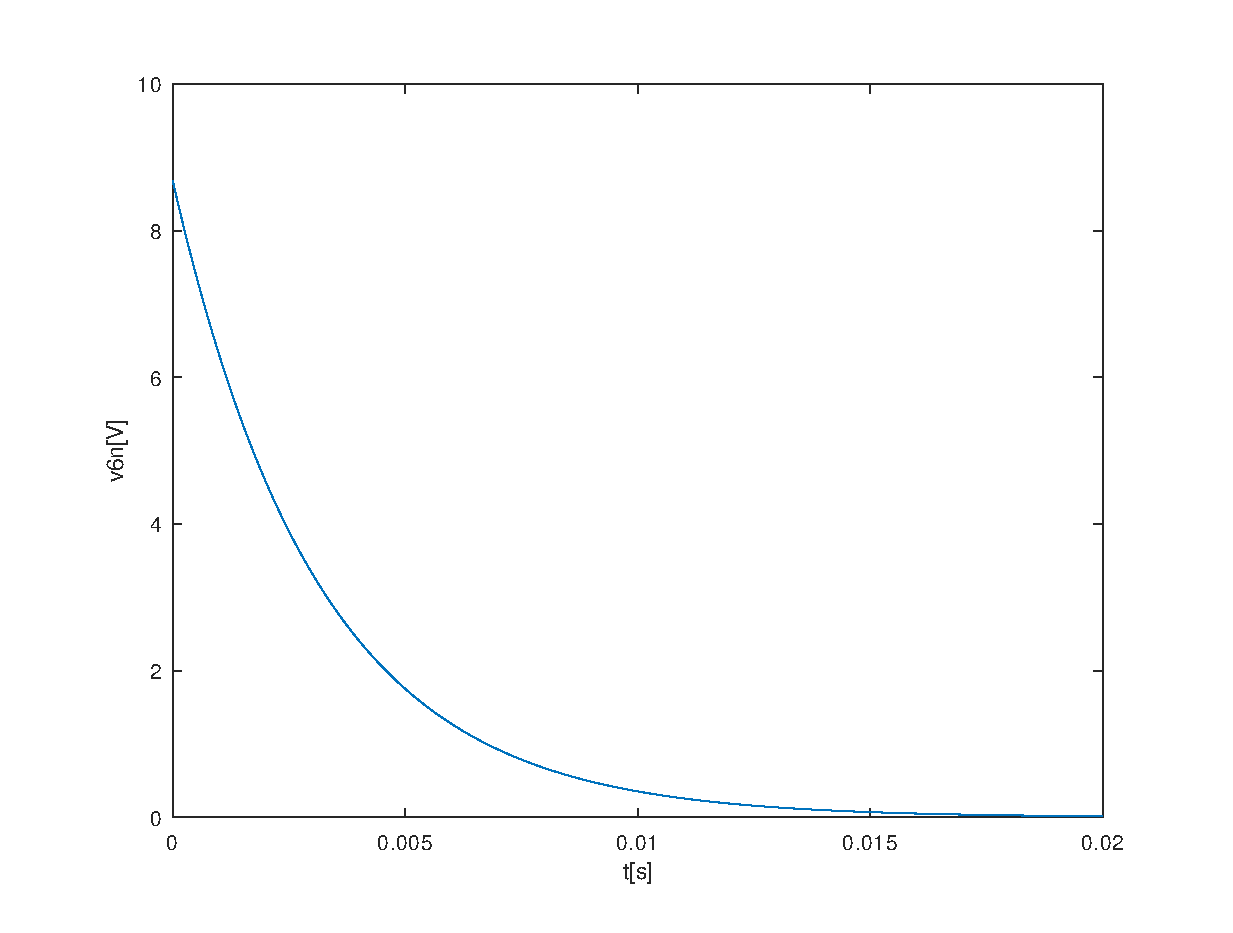
\includegraphics[width=0.4\linewidth]{t2-t3.eps}
\caption{The original circuit, with some current directions added.}
\label{cfergter}
\end{figure}


\subsection{Determining the Forced Solution for $V_6(t)$}

\begin{table}[h]
  \centering
  \begin{tabular}{|l|r|}
    \hline    
    {\bf Name} & {\bf Voltages [V]} \\ \hline
    V0real & -2.7665952e-17\\\hline V1real & 1.0000000e+00\\\hline V2real & 9.5304035e-01\\\hline V3real & 8.5357688e-01\\\hline V5real & 9.5987855e-01\\\hline V6real & -5.6551340e-01\\\hline V7real & -3.8119691e-01\\\hline V8real & -5.6984862e-01\\\hline 


V0imag & -2.4572302e-32\\\hline V1imag & 0.0000000e+00\\\hline V2imag & 5.8138780e-16\\\hline V3imag & 1.8224151e-15\\\hline V5imag & 4.9606606e-16\\\hline V6imag & -8.5097837e-02\\\hline V7imag & -1.9700289e-16\\\hline V8imag & -2.9449826e-16\\\hline 
  \end{tabular}
  \caption{T2 1) Node Analysis Computation Results: Currents (A) computed using ohms law}
  \label{tab:nodeVoltages2}
\end{table}

\subsection{Determining the Final Total Solution for $V_6(t)$}

\begin{figure}[h] \centering
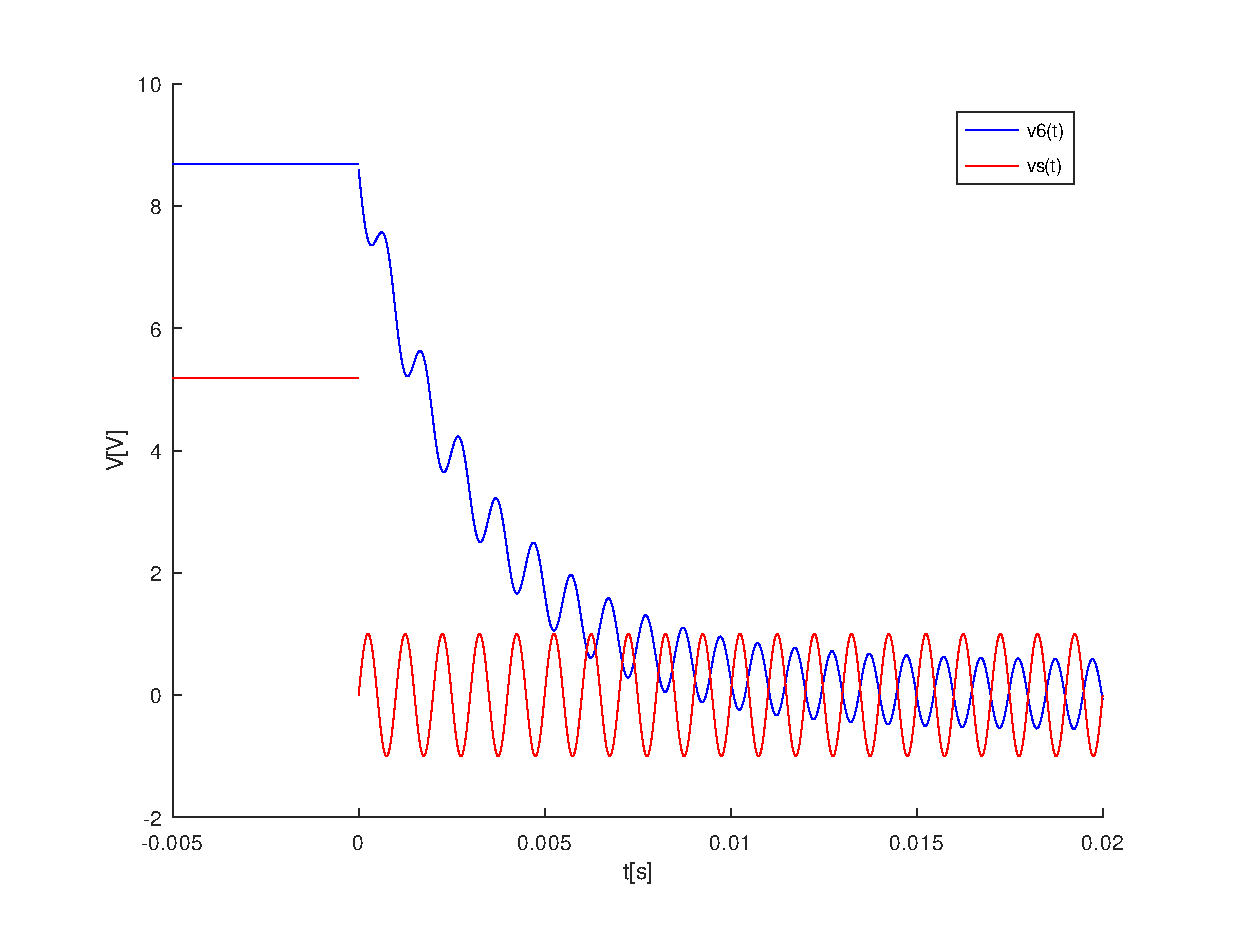
\includegraphics[width=0.4\linewidth]{t2-t5.eps}
\caption{The original circuit, with some current directions added.}
\label{cfergter}
\end{figure}


\subsection{NEM PERCEBO O QUE RAIO ELES QUEREM AQUI}

\begin{figure}[h] \centering
\includegraphics[width=0.4\linewidth]{t2-t6-mag.eps}
\caption{The original circuit, with some current directions added.}
\label{cfergter}
\end{figure}

\begin{figure}[h] \centering
\includegraphics[width=0.4\linewidth]{t2-t6-fase.eps}
\caption{The original circuit, with some current directions added.}
\label{cfergter}
\end{figure}